\section{COVR}
\label{sCOVR}

\subsection{Introduction}
\label{ssCOVR_intro}

\hypertarget{sCOVRhy}{The}
COVR\index{COVR|textbf} module of NJOY is an editing module that
post processes the output of
\hyperlink{sERRORRhy}{ERRORR}\index{ERRORR} in a manner
analogous to the way
\hyperlink{sMATXSRhy}{MATXSR}\index{MATXSR} and
\hyperlink{sDTFRhy}{DTFR}\index{DTFR}
post process the output of
\hyperlink{sGROUPRhy}{GROUPR}\index{GROUPR}.  COVR performs
two quite separate functions using the multigroup covariance
file\index{covariances} from
\hyperlink{sERRORRhy}{ERRORR} as input.  First, it can
prepare a new covariance library in a highly compressed
card-image format, which is suitable for use as input to sensitivity
analysis programs\cite{sensit,sensit-2}.\index{sensitivity analysis}
Data in this form can also be copied to the system output file
to obtain a compact printed summary of an
\hyperlink{sERRORRhy}{ERRORR} run without using
the sometimes bulky long-print option in
\hyperlink{sERRORRhy}{ERRORR}.  Such a summary
can also provide information on standard deviations and correlation
coefficients, neither of which are printed by
\hyperlink{sERRORRhy}{ERRORR}.  The second
main function of COVR is to produce publication-quality
plots\cite{LaBauve} of the multigroup covariance information.
\index{plotting}
\index{plotting!covariance data}

This chapter describes the COVR module in NJOY2016.0.

\subsection{Production of Boxer-Format Libraries}
\label{ssCOVR_Boxer}

As discussed in the
\hyperlink{sERRORRhy}{ERRORR} section of this manual, the
output file of that module contains the group structure, cross
sections, and either absolute (\cword{irelco}=0) or relative
(\cword{irelco}=1) covariances for one or more materials, in either
card-image or NJOY blocked-binary form.  If the COVR user-input
parameter \cword{nout} is greater than zero, COVR reads an
\hyperlink{sERRORRhy}{ERRORR}
output file from unit \cword{nin} and produces a new multigroup
covariance library on unit \cword{nout}.  COVR performs only sorting
and reformatting operations on the
\hyperlink{sERRORRhy}{ERRORR} data.

In COVR, as well as
\hyperlink{sERRORRhy}{ERRORR}, the ENDF energy ordering is followed.  That
is, low group indices correspond to low energies, high indices to high
energies.  Regarding group structures, in the library mode of
operation COVR (like
\hyperlink{sERRORRhy}{ERRORR}) makes extensive use of external (disk)
storage so that even on machines that have a relatively small central
memory very large group structures (up to 640 groups) can be handled
successfully.  (See, however, the comments at the end of
Section \ref{ssCOVR_plot}
regarding group-number limitations in the plot mode.)

The material and reaction coverage of COVR post-processing is
determined by a set of reaction pairs \cword{(mat,mt;mat1,mt1)}
supplied by the user (see input Card 4 in the input instructions
and the corresponding discussion that follows in Section \ref{ssCOVR_inp}).
At the beginning of the output library, the group structure is given.  Then,
for each specified reaction pair, the output library contains either a
covariance matrix or a correlation matrix, depending on the output
option (\cword{matype}) selected.  In the case that covariances are
requested (\cword{matype}=3), the type of data on \cword{nout}
(absolute {\it vs.} relative) is governed by the covariance type present
on \cword{nin}.   In addition, whenever \cword{mat1}$=$\cword{mat} and
\cword{mt1}$=$\cword{mt}, the group-cross-section vector and the
(absolute/relative) standard-deviation vector for that particular
reaction are written to \cword{nout} just before the matrix itself.
All data (group structure, cross sections, standard deviations, and
matrices) are written to \cword{nout} using a highly compressed,
card-image format.

The design of this format, called the BOXER format\index{BOXER format},
proceeds from a simple fact: as discussed in the
\hyperlink{sERRORRhy}{ERRORR} section of this
manual, most of the ENDF covariance formats define certain rectangular
regions (boxes) in energy ``space,'' over which the relative covariance
is constant. (The ENDF format allowing a constant absolute
covariance is only rarely used.)  The coordinate axes of the
two-dimensional energy space in question are $E_{x}$ and $E_{y}$, where
$x$ and $y$ indicate the particular reaction pair to which the ENDF
covariances apply.  Because of this feature of the basic evaluations,
one expects that an element of a multigroup relative covariance matrix,
derived from the ENDF data for a given reaction pair, frequently will
be identical either to the element before it in the same row ($E_{x}$
constant, $E_{y}$ varying) or to the element above it in the same
column ($E_{y}$ constant, $E_{x}$ varying).  Thus, the Boxer format
allows a combination of horizontal and vertical repeat
operations.

Even though the
\hyperlink{sERRORRhy}{ERRORR} output format already suppresses zero
covariances, very large data compression factors can be achieved in
transforming data from the
\hyperlink{sERRORRhy}{ERRORR} format to the Boxer format.  As one
example, the
\hyperlink{sERRORRhy}{ERRORR} output file for a particular 137-group
reactor-dosimetry library\cite{multigroup} contained 38 000 card
images, while the corresponding COVR output file contained fewer than
1000 card images.

In the BOXER format, data are stored as a list of numerical data values
({\it e.g.}, relative covariances), together with a list of integers
that control the loading of these data into the reconstructed array
$C(i,j)$.  A negative control integer, $-n$, indicates that the next
value in the data list is to be loaded into the next $n$ columns
($j$-locations) of the current row of $C(i,j)$.  A positive integer
$m$, on the other hand, means that, for the next $m$ $j$-values, the
value to be loaded is to be carried down from the row above,
\begin{equation}
C(i,j) = C(i{-}1,j)\:.
\end{equation}

\noindent
For the first row $(i = 1)$, the row above is defined to contain all zeros.

In constructing the compressed data set in subroutine \cword{press},
the choice between using the ``repeat-new-value'' method or
the ``carry-down'' method is made dynamically on the basis of taking
the longest possible step.  If $m = n$, the carry-down method is
chosen, as it does not require an entry in the data list.

As an additional compression feature of the format, one may indicate by
a ``flag'' that the matrix $C(i,j)$ is symmetric; hence, explicit
instructions are provided in the compressed data library for the
reconstruction  of only the upper right triangle of $C(i,j)$.  These
various aspects of the Boxer format are illustrated by a simple example
in Fig.~\ref{boxing}.  Here $a,b,c$ and $d$ are arbitrary, nonzero,
unequal data values.

\begin{figure}[htb]

\begin{center}
\underline{Original Data Set}
%\end{center}

\setlength{\unitlength}{.4in}
\begin{picture}(10,8)(-1,0)
\put(4,7){$j~\rightarrow$}
\put(.5,3.5){$i$}
\put(.5,3.0){$\downarrow$}
\put(2,6){$a$}
\put(1.5,5.5){\line(1,0){1}}
\put(2.5,5.5){\line(0,-1){1}}
\put(3,6){$a$}
\put(4,6){$b$}
\put(5,6){$b$}
\put(6,6){$0$}
\put(7,6){$0$}
\put(2,5){$a$}
\put(3,5){$a$}
\put(2.5,4.5){\line(1,0){1}}
\put(3.5,4.5){\line(0,-1){1}}
\put(4,5){$b$}
\put(5,5){$b$}
\put(6,5){$0$}
\put(7,5){$0$}
\put(2,4){$b$}
\put(3,4){$b$}
\put(4,4){$b$}
\put(3.5,3.5){\line(1,0){1}}
\put(4.5,3.5){\line(0,-1){1}}
\put(5,4){$b$}
\put(6,4){$0$}
\put(7,4){$0$}
\put(2,3){$b$}
\put(3,3){$b$}
\put(4,3){$b$}
\put(5,3){$b$}
\put(4.5,2.5){\line(1,0){1}}
\put(5.5,2.5){\line(0,-1){1}}
\put(6,3){$0$}
\put(7,3){$0$}
\put(2,2){$0$}
\put(3,2){$0$}
\put(4,2){$0$}
\put(5,2){$0$}
\put(6,2){$c$}
\put(5.5,1.5){\line(1,0){1}}
\put(6.5,1.5){\line(0,-1){1}}
\put(7,2){$c$}
\put(2,1){$0$}
\put(3,1){$0$}
\put(4,1){$0$}
\put(5,1){$0$}
\put(6,1){$c$}
\put(7,1){$d$}
\end{picture}
%\end{center}


%\begin{center}
\underline{Boxer Format, Symmetry Flag Off}
%\end{center}

\begin{picture}(10,2.5)(0,0)
\put(2,2){$a$}
\put(3,2){$b$}
\put(4,2){$b$}
\put(5,2){$0$}
\put(6,2){$c$}
\put(7,2){$d$}
\put(1.8,1){$-2$}
\put(2.8,1){$-2$}
\put(4,1){$8$}
\put(4.8,1){$-4$}
\put(6,1){$8$}
\put(6.8,1){$-4$}
\put(7.8,1){$-2$}
\put(9,1){$5$}
\put(9.8,1){$-1$}
\end{picture}
%\end{center}


%\begin{center}
\underline {Boxer Format, Symmetry Flag On}
%\end{center}

\begin{picture}(10,2.5)(-1,0)
\put(2,2){$a$}
\put(3,2){$b$}
\put(4,2){$c$}
\put(5,2){$d$}
\put(1.8,1){$-2$}
\put(2.8,1){$-2$}
\put(4,1){$14$}
\put(4.8,1){$-2$}
\put(5.8,1){$-1$}
\end{picture}
\end{center}

\caption{Illustration of Boxer format}
\label{boxing}

\end{figure}


Before the data values are tested in \cword{press}\index{press@{\ty press}}
to see if they are indeed equal, the \hyperlink{sNJOYhy}{NJOY} utility
\cword{sigfig}\index{sigfig@{\ty sigfig}}\index{significant figures}
is called to round off the trailing digits that would not appear on
the formatted output anyway.  Relative covariances, for example, are
written to \cword{nout} in 1P8E10.3 format, which has only four
significant figures.  Thus, the three data values 0.036126, 0.036130,
and 0.036134 would all be judged to be equal by this logic.

\subsection{Generation of Plots}
\label{ssCOVR_plot}

The COVR plot mode, which is requested by specifying \cword{nout}=0, is
used to generate publication-quality plots of multigroup covariance
data from a card-image or binary
\hyperlink{sERRORRhy}{ERRORR}\index{ERRORR} output file.
Examples of plots produced by COVR can be seen in the
\hyperlink{sERRORRhy}{ERRORR} section
of this manual.  In addition to their usefulness in preparing
publications, the plots have proved to be a useful tool for checking
the reasonableness and mechanical correctness of new covariance
evaluations.  One can, for example, execute
\hyperlink{sERRORRhy}{ERRORR} and COVR in tandem,
using the evaluator's energy grid as the user group structure
(\hyperlink{sERRORRhy}{ERRORR} input option \cword{ign}=19).  The
output of such a run
is a series of plots showing all important features of the covariance
evaluation.

As can be seen in the examples mentioned above, each plot contains a
shaded contour map of the correlation matrix.  If black \& white plots
are needed, positive-correlation regions are shaded with parallel
straight lines (hatching), while negative correlations are indicated
by cross-hatching.  When color is requested (see the second card in the
input instructions, the positive correlations are represented by shades
of green, and the negative correlations are represented by shades of red.
\index{plotting!correlation matrix}
\index{plotting!contour plots}
The plots also contain two additional inset graphs giving the energy
dependence of the associated standard deviation vectors.
\index{plotting!standard deviation}
One of the vector plots is rotated by 90 degrees, so that the
logarithmic energy scales for the vector plots can be aligned with
the corresponding scales for the matrix plot.  When \cword{MAT}=\cword{MAT1}
and \cword{MT}=\cword{MT1}, we plot the cross section rather than repeating
the standard deviation plot.

This type of plot presents the covariance data in a more lucid manner
than most alternative plotting packages.  However, use of this option
does require the sophisticated capabilities of the
\hyperlink{sVIEWRhy}{VIEWR}\index{VIEWR}
module to create rotated subplots and to fill regions with colors or
hatching patterns.  See the \hyperlink{sVIEWRhy}{VIEWR} section
of this report for more details.

Just as in the library mode, the material and reaction coverage of the
sequence of plots generated in the plot mode is determined by the
reaction pairs specified by the user on input Card 4.  Other input,
specific to the generation of plots, is described in Section~\ref{ssCOVR_inp}.
We next discuss some aspects of the plot-generation coding.

After a covariance matrix is read in subroutine
\cword{covard}\index{covard@{\ty covard}}, it is
converted to a correlation matrix in subroutine
\cword{corr}\index{corr@{\ty corr}}.  The
correlation matrix is then scanned in subroutine
\cword{matshd}\index{matshd@{\ty matshd}} to find a set of boundary
curves that divide $E_{x} - E_{y}$ energy space into a small number of
connected regions of nearly constant correlation strength.  Here the
phrase ``nearly constant'' refers to the subdivision of the range of
possible correlation values $(-1.0$ to $+1.0)$ into a number of
equal-width bands, the fineness of the subdivision being controlled
by the user-input parameter \cword{ndiv}.  Two regions have nearly
equal correlations if the correlations fall into the same band.  As
each boundary curve is located, the enclosed region is shaded (with a
line density proportional to the band correlation magnitude) with
direct writes to the \hyperlink{sVIEWRhy}{VIEWR} file.

The algorithm used to find the maximum extent of a region of nearly
constant correlation is best described by referring to the simple
example in Fig.~\ref{shade}.  After locating the upper left corner of a new
correlation region, for example at point $a$ in the figure, the search
proceeds as far as possible down the first column ($E_{y}$ held
constant) to point $b$.  New columns are scanned in the same way:
$c-d$, $e-f$, $g-h$.  Having found that the pattern does continue into
column $e-f$, for the sake of simplicity, the algorithm ignores the
possibility of additional, disjoint, continuations of the pattern
elsewhere in the same column (such as at $e'-f'$), and
region I is ended at $h$.  (Region II will be found and correctly
shaded at a later stage of the calculation.)

\begin{figure}[htb]\centering
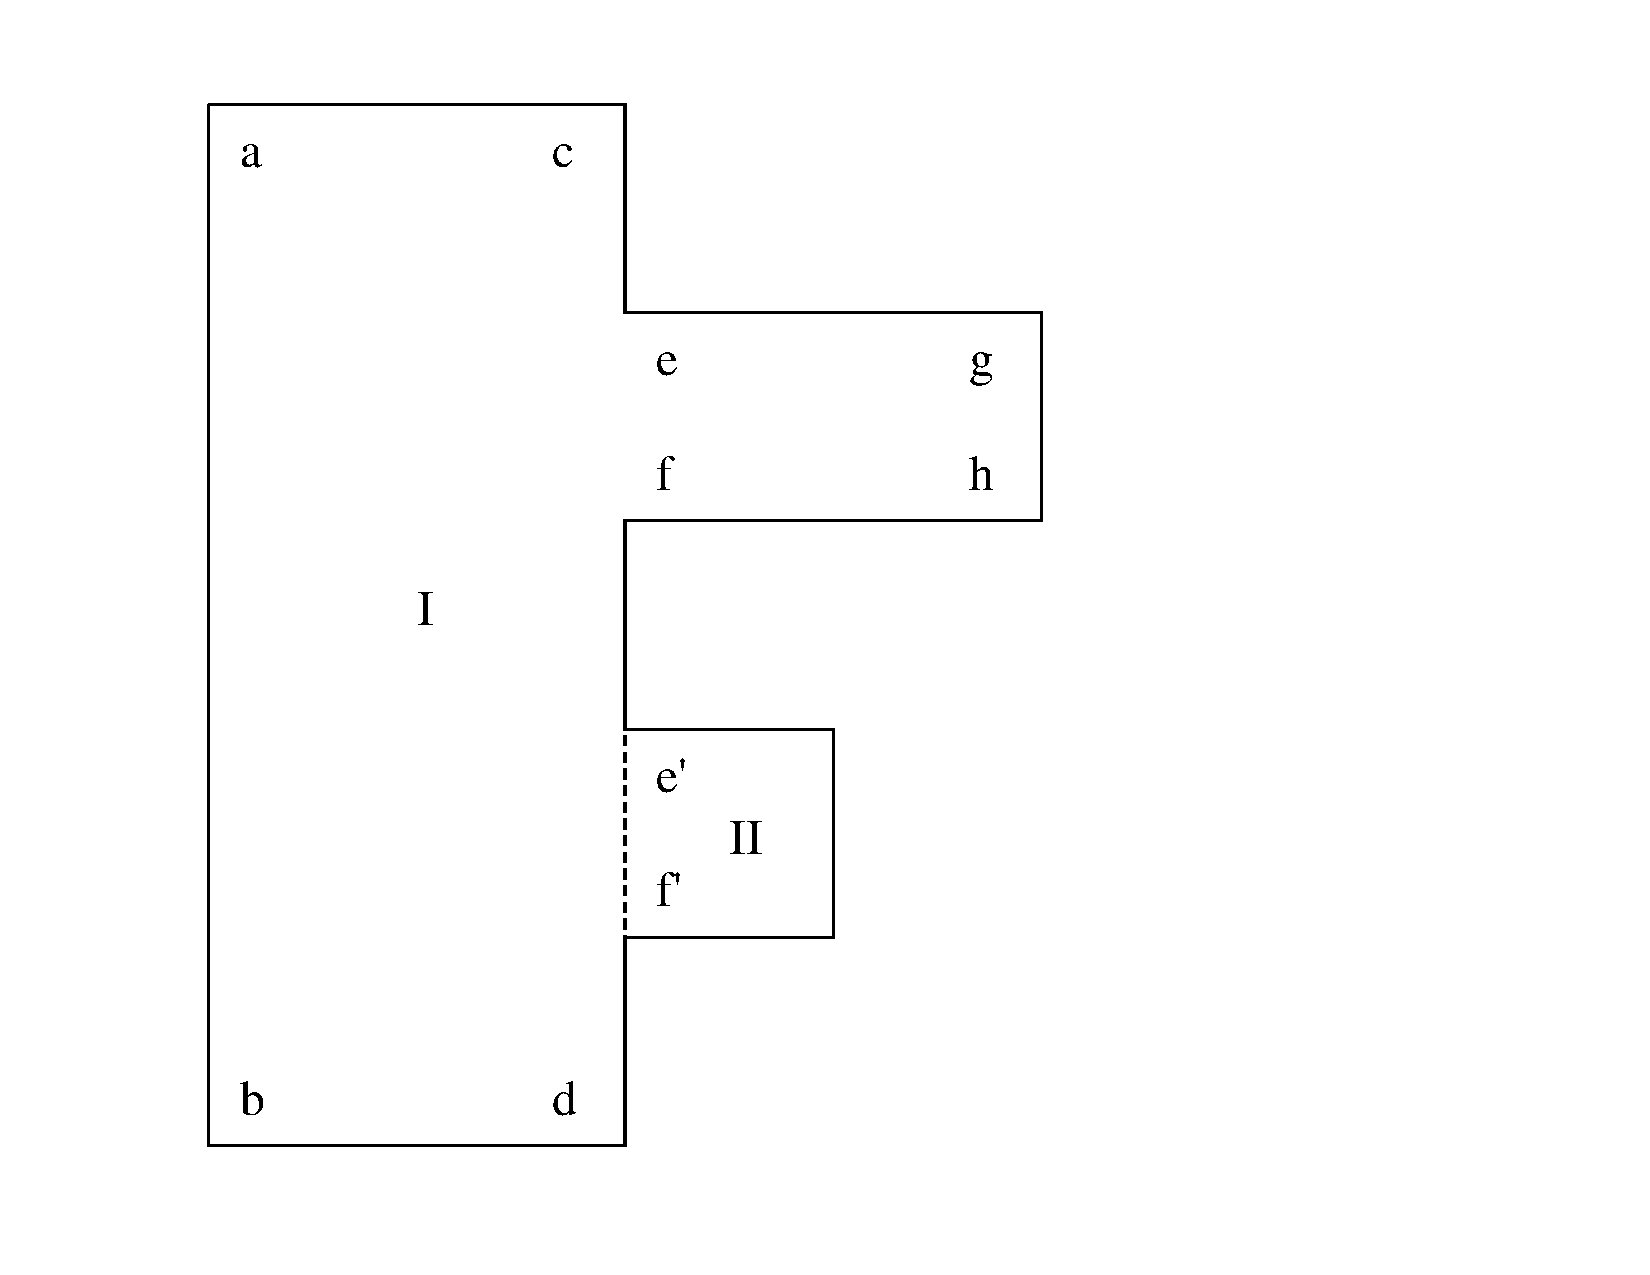
\includegraphics[keepaspectratio, height=4.0in, angle=0]{figs/covr1ack}
\caption[Pattern-search logic in used in COVR's subroutine
 matshd]{Pattern-search logic in subroutine matshd.}
\label{shade}
\end{figure}

As the plot option is presently coded, the entire correlation matrix
must reside in memory during the pattern-search operation just
described.

\subsection{Input Instructions for COVR}
\label{ssCOVR_inp}

As an aid to discussions of the user input to COVR, we list below the
input instructions that appear as comment cards at the beginning of the
current version of this module.  It is always advisable to consult the
comment-card instructions embedded in the version of the code actually
being used and not to rely on the instructions published in any
document, including this one.  Following the listing are further
remarks on several of the input items; the remarks supplement the
comment cards below.  See especially the lengthy discussion of the
parameters on Card 4.
\index{COVR!COVR input}
\index{input!COVR}

\small
\begin{ccode}

   !---input specifications (free format)---------------------------
   !
   !  card 1
   !     nin            input tape unit
   !     nout           output tape unit
   !                    (default=0=none)
   !     nplot          viewr output unit
   !                    (default=0=none)
   !
   !   ---cards 2, 2a, and 3a for nout.ne.0 only (plot option)
   !
   !  card 2
   !     icolor          select color or monochrome style
   !                       0=monochrome (uses cross hatching)
   !                       1=color background and contours
   !                       2=color background and contours plus
   !                         card 2' follows.
   !                       (default=0)
   !  card 2' (only when icolor=2)
   !     nlev,(tlev(i),i=1,nlev)
   !                     defines the number of correlation matrix
   !                     intervals and their boundaries.  Zero is
   !                     assumed as the lower limit of the first
   !                     boundary, but the User must specify unity
   !                     as the upper limit of the last boundary.
   !                     nlev is a positive integer .le. 9.
   !                     default values (when icolor=1) are:
   !                       6,0.001,0.1,0.2,0.3,0.6,1.0
   !  card 2a
   !     epmin          lowest energy of interest (default=0.)
   !  card 3a
   !     irelco         type of covariances present on nin
   !                    0/1=absolute/relative covariances
   !                    (default=1)
   !     ncase          no. cases to be run (maximum=40)
   !                    (default=1)
   !     noleg          plot legend option
   !                    -1/0/1=legend for first subcase only/
   !                    legend for all plots/no legends
   !                    (default=0)
   !     nstart         sequential figure number
   !                    0/n=not needed/first figure is figure n.
   !                    (default=1)
   !     ndiv           no. of subdivisions of each of the
   !                    gray shades (default=1)
   !
   !   ---cards 2b, 3b, and 3c for nout gt 0 (library option) only--
   !
   !  card 2b
   !     matype         output library matrix option
   !                    3/4=covariances/correlations
   !                    (default=3)
   !     ncase          no. cases to be run (maximum=40)
   !                    (default=1)
   !  card 3b
   !     hlibid         up to 6 characters for identification
   !  card 3c
   !     hdescr         up to 21 characters of descriptive
   !                    information
   !
   !   ---cards 4 for both options---
   !
   !  card 4
   !     mat            desired mat number
   !     mt             desired mt number
   !     mat1           desired mat1 number
   !     mt1            desired mt1 number
   !                    (default for mt, mat1 and mt1 are 0,0,0
   !                    meaning process all mts for this mat
   !                    with mat1=mat)
   !                    (neg. values for mt, mat1, and mt1 mean
   !                    process all mts for this mat, except for
   !                    the mt-numbers -mt, -mat1, and -mt1.  in
   !                    general, -n will strip both mt=1 and mt=n.
   !                    -4 will strip mt=1, mt=3, and mt=4, and
   !                    -62, for example, will strip mt=1, mt=62,
   !                    mt=63, ... up to and incl. mt=90.)
   !          repeat card 4 ncase times
   !
   ! note---if more than one material appears on the input tape,
   ! the mat numbers must be in ascending order.
   !
   !--------------------------------------------------------------------

\end{ccode}
\normalsize

\cword{icolor} \ldots\hspace{0.1in}This parameter is used to specify
creation of monochrome (cross-hatched) or color correlation matrix
plots.  Although the default setting is \cword{icolor}=0 (to produce
monochrome plots) the capabilities of modern printers and display
terminals makes creation of color plots the more common
option.  If \cword{icolor}=1 a default six-interval color pattern is
used when creating the correlation matrix; if \cword{icolor}=2 then
input card~2' is required where the user specfies the number of
color intervals (an integer, \cword{nlev}, where \cword{nlev} is a
positive non-zero integer $<$ 10) plus \cword{nlev} real numbers
that define the color boundaries, \cword{tlev(i)}, i=1,
\cword{nlev}.  \cword{tlev(\cword{nlev})} must be unity.  Users
are cautioned that use of too many intervals may require an
increase in the value of \cword{ipat} in \cword{subroutine matshd}.

\cword{epmin } \ldots\hspace{.1in}This parameter is used to eliminate
uninteresting energy regions from the correlation and standard
deviation plots, or to display high-energy regions with greater
resolution.

\cword{irelco } \ldots\hspace{.1in}This parameter must
match the value used in the \hyperlink{sERRORRhy}{ERRORR}
run that produced the covariances to be plotted.

\cword{ncase } \ldots\hspace{.1in}This is the number of cases, or
occurrences of Card 4.  See the discussion of input parameters
\cword{mat}, \cword{mt}, \cword{mat1}, and \cword{mt1} below.
Presently, \cword{ncase} is limited to 60.  Problems larger than this
can be run as a series of COVR jobs, each processing a batch of up to
60 cases.  See also the parameter \cword{nstart} below.

\cword{noleg } \ldots\hspace{.1in}``Legend'' here refers to the
gray-shading scale (key) as well as the figure caption.
\cword{noleg}=1 is used as a rough-draft mode to display plots
quickly.

\cword{nstart } \ldots\hspace{.1in}Unless \cword{nstart}=0, the plots
are assigned a sequential figure number, beginning at \cword{nstart},
and a list of figures is drawn on the final plot frame.

\cword{ndiv } \ldots\hspace{.1in}One gray-shade step equals 0.20 in
correlation magnitude if \cword{ndiv}=1.  Finer gradations are possible
with \cword{ndiv} greater than 1.  The plots appearing in the
\hyperlink{sERRORRhy}{ERRORR} section of this manual were
generated with \cword{ndiv}=2.

\cword{hlibid } \ldots\hspace{.1in}This is a 6-character string,
normally containing the name of the output covariance library.  It
is written on the header records present at the beginning of each
output data block.

\cword{hdescr } \ldots\hspace{.1in}This contains additional
information, for example, on where and when the library was produced;
it is also written on the data header records.

\cword{mat, mt, mat1, mt1 } \ldots\hspace{.1in}The information
contained in the output library or plot file is controlled by means of
these parameters on input Card 4.  If \cword{mt} is
positive, then a single covariance matrix for reaction
(\cword{mat,mt}) with reaction (\cword{mat1,mt1}) will be read from
\cword{nin} and processed.  On unit \cword{nin} (and, in the library
option, on unit \cword{nout}), the rapidly varying, or column,
index is the group index of (\cword{mat1,mt1}), and the slowly varying,
or row, index is the group index of (\cword{mat,mt}). ~If
\cword{mat1} is different from \cword{mat}, COVR will expect to find
separate materials (produced by separate
\hyperlink{sERRORRhy}{ERRORR} runs) for both
\cword{mat} and \cword{mat1} on \cword{nin}.  The \cword{mat} numbers
must occur on \cword{nin} in ascending order.  In the case of positive
\cword{mt}, the entries \cword{mat1}=0 and \cword{mt1}=0 are shorthand
for \cword{mat1}=\cword{mat} and \cword{mt1}=\cword{mt}, respectively.
If, on the other hand, \cword{mt} is zero, negative, or
defaulted, Card 4 becomes a kind of macro-instruction that
is expanded by subroutine \cword{expndo} into a request for many
(\cword{mt, mt1}) pairs, all  with \cword{mat1}=\cword{mat}.  If, for example,
Card 4 contains the entry

\small
\begin{ccode}

     MAT/

\end{ccode}
\normalsize

\noindent
or, equivalently,

\small
\begin{ccode}

     MAT 0 0 0/

\end{ccode}
\normalsize

\noindent
first the cross-section file, \cword{MF}$ = $\cword{3}, for material
\cword{MAT} is read from the input covariance tape on unit
\cword{nin} to obtain the list of reactions present.  Then, all
possible reaction combinations (\cword{mt, mt1}) are formed in ENDF
order.  Thus, for example, if the reactions present are \cword{MT}$ =
$\cword{1, 2, 3}, and \cword{16}, then the behavior of the code is the
same as if the following input were specified:

\small
\begin{ccode}

     MAT 1 0 1/
     MAT 1 0 2/
     MAT 1 0 3/
     MAT 1 0 16/
     MAT 2 0 2/
     MAT 2 0 3/
     MAT 2 0 16/
     MAT 3 0 3/
     MAT 3 0 16/
     MAT 16 0 16/

\end{ccode}
\normalsize

\noindent
Because of the clear labor-saving advantage of this feature, especially if
there are many reactions, enhancements have been added to permit its use
in the additional situation in which many, but not all, combinations are
desired.  As discussed in some detail in the input instructions, it is
possible to strip selected reactions out of the list before the
(\cword{mt, mt1}) combinations are formed.  For example, if the reactions
present are once again 1, 2, 3, and 16, then a Card 4 containing

\small
\begin{ccode}

     MAT -3/

\end{ccode}
\normalsize

\noindent
would produce the same output as the following three cards:

\small
\begin{ccode}

     MAT 2 0 2/
     MAT 2 0 16/
     MAT 16 0 16/

\end{ccode}
\normalsize

\noindent
The stripping of the higher inelastic levels, mentioned in the input
instructions, is useful because \hyperlink{sERRORRhy}{ERRORR}
automatically resets the
highest user-group energy to 20 MeV whenever \cword{IREAD}=0, and this
can result in the inclusion of unwanted high-threshold reactions on the
\hyperlink{sERRORRhy}{ERRORR} output file.

For one of several reasons, a requested reaction pair
(\cword{mat,mt; mat1,mt1}) may be absent from the COVR output.
The usual reason that this occurs is that the normal \cword{iread} option
for the \hyperlink{sERRORRhy}{ERRORR} module is \cword{iread}=0,
and this results in the generation of an output matrix for every
possible reaction-pair combination.  For those combinations that
do not occur in the ENDF evaluation, the
\hyperlink{sERRORRhy}{ERRORR} output matrix contains only
zeroes.  These null matrices are omitted at the COVR output stage,
in both the library and plot modes.

Additionally, in the plot mode, the correlations may be nonzero, but
everywhere less than \cword{0.2/ndiv} in absolute magnitude.  In this
case, the entire correlation plot would consist of a single blank region.
These rather uninteresting plots having small correlations are also
omitted from the plot file.  A final, similar category is the class of
``empty'' plots.  Because parallel lines to achieve a gray effect
when color is not used have limited resolution, there
is clearly some lower limit, for a given value of the correlation
magnitude, on the physical size of a region that can be sensibly shaded.
COVR does not attempt to shade regions that are smaller than this limit.
If a correlation matrix does contain some plottable data (magnitudes
exceeding \cword{0.2/ndiv}), but all plottable regions are smaller than
the size limit discussed above, then an empty plot will be generated on
the plot file.  As a convenience in discarding these empty plots at the
time a report is produced, no caption is written on such plots and the
figure number is not advanced.  Also, these plots are omitted from
the list of figures prepared at the end of a plot run.  (See the
discussion of user-input parameter \cword{nstart}.)

In the library mode, each omission of a requested, but null, matrix is
noted on the \cword{output} file with an informative diagnostic.  In the
plot mode, a summary table is printed at the end of the run to identify
all requested matrices that were omitted because they were null or
small, as well as those that were plotted, but empty.


\subsection{COVR Example Problem}
\label{ssCOVR_example1}

In this section we discuss the production of a particular COVR output
library, both to illustrate the input and as a supplement to the
general discussion of BOXER format libraries in  Section~\ref{ssCOVR_Boxer}.
In the \hyperlink{sERRORRhy}{ERRORR} chapter of this report
(the second input set in Section~\ref{ssERRORR_inp}),
we gave the complete NJOY input for producing a 7-reaction,
30-group covariance library in \hyperlink{sERRORRhy}{ERRORR}
output format for $^{12}$C.  By appending the following lines to
that input (just before the \cword{stop} card), one can produce,
in addition, a 2-reaction COVR output library in BOXER format.

\small
\begin{ccode}

     covr
     -23 24/
     3 3/
     '  LIB'/
     'MAT1306 COVR EXAMPLE'/
     1306 2 0 2/
     1306 2 0 4/
     1306 4 0 4/

\end{ccode}
\normalsize

\noindent
The resulting library occupies only 49 lines and is listed below.

%\begin{ccode}
\small
\begin{verbatim}
0    LIB-A- 30 MAT1306 COVR EXAMPLE  1306   2 1306   2  31 10  31  3   0  31   1
 1.390E-04 1.520E-01 4.140E-01 1.130E+00 3.060E+00 8.320E+00 2.260E+01 6.140E+01
 1.670E+02 4.540E+02 1.235E+03 3.350E+03 9.120E+03 2.480E+04 6.760E+04 1.840E+05
 3.030E+05 5.000E+05 8.230E+05 1.353E+06 1.738E+06 2.232E+06 2.865E+06 3.680E+06
 6.070E+06 7.790E+06 1.000E+07 1.200E+07 1.350E+07 1.500E+07 1.700E+07
 -1 -1 -1 -1 -1 -1 -1 -1 -1 -1 -1 -1 -1 -1 -1 -1 -1 -1 -1 -1 -1 -1 -1 -1 -1 -1
 -1 -1 -1 -1 -1
1    LIB-A- 30 MAT1306 COVR EXAMPLE  1306   2 1306   2  23 10  23  3   0  30   1
 4.739E+00 4.738E+00 4.735E+00 4.729E+00 4.712E+00 4.676E+00 4.579E+00 4.332E+00
 4.002E+00 3.619E+00 3.103E+00 2.477E+00 1.998E+00 1.820E+00 1.710E+00 2.256E+00
 1.447E+00 9.921E-01 8.223E-01 7.627E-01 8.631E-01 8.228E-01 8.845E-01
 -8 -1 -1 -1 -1 -1 -1 -1 -1 -1 -1 -1 -1 -1 -1 -1 -1 -1 -1 -1 -1 -1 -1
2    LIB-A- 30 MAT1306 COVR EXAMPLE  1306   2 1306   2  18 10  18  3   0  30   1
 2.000E-03 1.964E-03 4.583E-03 3.822E-03 4.583E-03 4.288E-03 3.730E-03 4.141E-03
 6.501E-03 1.011E-02 9.558E-03 9.981E-03 1.806E-02 1.854E-02 3.296E-02 3.760E-02
 4.255E-02 7.632E-02
 -9 -1 -5 -1 -1 -1 -1 -1 -1 -1 -1 -1 -1 -1 -1 -1 -1 -1
3    LIB-A- 30 MAT1306 COVR EXAMPLE  1306   2 1306   2  43 10  58  4   0  30   0
 4.000E-06 2.797E-06 3.856E-06 6.317E-06 4.613E-06 2.407E-06 1.229E-06 2.100E-05
 1.534E-05 8.000E-06 4.087E-06 1.461E-05 1.366E-05 2.100E-05 1.838E-05 9.004E-06
 1.391E-05 8.934E-06 1.715E-05 4.447E-06 4.227E-05 4.373E-05 2.446E-05 1.980E-05
 1.223E-05 1.022E-04 6.116E-05 4.048E-05 2.500E-05 9.136E-05 4.572E-05 9.962E-05
 6.641E-05 6.308E-05 3.260E-04 1.614E-04 3.437E-04 1.086E-03 4.250E-04 1.413E-03
 7.052E-04 1.811E-03 5.825E-03
  -9  -1 224  -1  -5  -1  -4  -1   9  -5  -1  -4  -1  79  -1  -1  13  -1  13  -1
  -1  11  -1  -1  10  -1  -1   9  -1  -1  -1  -1  -6  -1  -1  -1  -6  -1  -1   6
  -1  -1  -1   4  -1  -1   4  -1   4  -1  -2   1  -1  -1   1  -1   1  -1
3    LIB-A- 30 MAT1306 COVR EXAMPLE  1306   2 1306   4  38 10  47  4   0  30  30
-1.106E-04-4.897E-05-3.047E-05-2.164E-05-2.630E-05-2.337E-05-2.192E-05-2.261E-04
-1.001E-04-6.228E-05-4.423E-05-5.376E-05-4.777E-05-4.481E-05-1.441E-03-2.659E-04
-1.571E-04-1.210E-03-1.305E-03-4.021E-04-1.131E-03-6.462E-04-8.562E-04-2.261E-04
-1.001E-04-6.228E-05-1.922E-03-9.140E-04-8.121E-04-7.520E-04-3.040E-03-1.348E-03
-1.517E-03-3.460E-03-4.423E-05-5.376E-05-4.777E-05-1.044E-02
 623  -1  -1  -1  -1  -1  -1  -1  23  -1  -1  -1  -1  -1  -1  -1  53  -1  -1  -1
  27  -1  -1  -1  27  -1  -1  -1  27  -1  -1  -1  -1  -1  -1  27  -1  -1  -1  28
  -1  -1  27  -1  -1  -1  -1
1    LIB-A- 30 MAT1306 COVR EXAMPLE  1306   4 1306   4   7 10   8  3   0  30   1
 6.091E-02 2.478E-01 3.301E-01 4.310E-01 4.013E-01 4.306E-01 4.935E-01
 23 -1 -1 -1 -1 -1 -1 -1
2    LIB-A- 30 MAT1306 COVR EXAMPLE  1306   4 1306   4   7 10   8  3   0  30   1
 2.499E-01 1.085E-01 9.724E-02 9.806E-02 1.358E-01 1.263E-01 2.177E-01
 23 -1 -1 -1 -1 -1 -1 -1
3    LIB-A- 30 MAT1306 COVR EXAMPLE  1306   4 1306   4  28 10  29  4   0  30   0
 6.245E-02 7.530E-03 3.823E-03 1.154E-03 1.338E-03 1.211E-03 1.155E-03 1.176E-02
 2.311E-03 5.938E-04 6.451E-04 5.843E-04 5.578E-04 9.455E-03 1.887E-03 4.735E-04
 4.295E-04 4.106E-04 9.617E-03 1.872E-03 1.670E-03 3.033E-04 1.844E-02 5.214E-03
 3.493E-04 1.596E-02 5.253E-03 4.741E-02
 437  -1  -1  -1  -1  -1  -1  -1  -1  -1  -1  -1  -1  -1  -1  -1  -1  -1  -1  -1
  -1  -1  -1  -1  -1  -1  -1  -1  -1
\end{verbatim}
\normalsize
%\end{ccode}

Note that the header card at the start of each data block contains an
integer \cword{itype}, specifying the type of data contained in the
current block, a 12-character library name (``\cword{LIB-A- 30}'' in
this case), 21 characters of user-supplied descriptive information,
\cword{mat, mt, mat1, mt1}, and a set of 7 integers.  The meaning of
the various values of \cword{itype} is as follows: 0 = group
boundaries, 1 = cross sections, 2 = standard deviations, 3 =
covariances, and 4 = correlations.  The library name is generated within
COVR by adding either ``-A-" (for a covariance library) or
``-B-" (for a correlation library), together with the number of
energy groups, to the user-supplied library name \cword{hlibid}.  (The
\hyperlink{sERRORRhy}{ERRORR} input option \cword{ign}=3 used in
this example specifies a built-in 30-group structure).  The final
seven integers on the header card indicate the number and format
of the data values, the number and format of the control integers
(called {\it ``m''} and {\it ``-n''} in the discussion in
Section~\ref{ssCOVR_Boxer}), a data paging flag, and the
dimensions of the reconstructed data array, $C(i,j)$.

In order to clarify the process of reconstructing a full matrix from
data in BOXER format, we list in Section~\ref{ssCOVR_retrieval} a short
retrieval program, BOXR.  With very few modifications, this program could be
incorporated into a sensitivity analysis program, for example, to allow
direct access to covariance libraries\cite{COVFILS2} in this compact
format.  Alternatively, it could be used to translate COVR libraries
into other desired forms.  In any case, an examination of the retrieval
program should clarify the meaning of the various integer parameters on
the header cards in a COVR output library.

\subsection{Error Messages}
\label{ssCOVR_err}

\begin{description}
\begin{singlespace}

\item[\cword{error in covr***requested too many cases.}]~\par
  \cword{ncase} is limited to 40.  Note that a case refers to one
  input Card 4, which may request processing of either a single reaction
  pair or a whole series of reaction pairs.  See input instructions for
  Card 4 and the comments that follow.

\item[\cword{error in expndo***storage exceeded.}]~\par
  Should not occur since array space is allocated based upon known
  storage needs.

\item[\cword{error in corr***group structures do not agree.}]~\par
  This problem should not occur.

\item[\cword{error in covard***storage exceeded.}]~\par
  Should not occur since array space is allocated based upon known
  storage needs.

\item[\cword{error in covard***did not find file 77 subsection...}]~\par
  Requested reaction y of the current x-y pair is not found on \cword{nin}.

\item[\cword{error in trunc***bad data.}]~\par
  Either all cross sections are very small (less than
  \cword{xslim} = $10^{-4}$ barn) or \cword{epmin} is larger than
  the highest group boundary.

\item[\cword{error in matshd***ipat gt 99999.}]~\par
  Maximum number of correlation patterns is 99999.  Reduce \cword{ndiv} to
  1 or raise \cword{epmin} in order to reduce the complexity of the
  correlation plot.

\item[\cword{error in matshd***storage exceeded.}]~\par
  \cword{nwig}=2*(\cword{ixmax}+1)+600 words are available for storing the
  boundary curve of a constant-correlation region.  This will not be
  exceeded for any practical number of groups \cword{ixmax}.

\item[\cword{error in level***coefficient = --- out of range.}]~\par
  The absolute magnitude of a computed correlation coefficient is greater
  than 2.  The input covariance file may be faulty.

\item[\cword{error in finds***mat --- mf --- mt --- not on tape.}]~\par
  Requested reaction x of the current x-y pair is not found on \cword{nin}.

\item[\cword{error in press***storage exceeded.}]~\par
  This problem should not occur.

\item[\cword{error in press***matrix not symmetric....}]~\par
  Symmetric-matrix format is requested for a matrix that is asymmetric.
  This problem should not occur.

\item[\cword{error in setfor***nvf (= ---) or ncf (= ---) is illegal.}]~\par
  This problem should not occur.

\end{singlespace}
\end{description}

\subsection{Input/Output Units}
\label{ssCOVR_IO}

The following logical units are used:
\begin{description}
\begin{singlespace}

\item[10]   \cword{nin} in \cword{corr} and \cword{covard, nscr} in
other routines.  These units are used to extract either one or two (if
\cword{mat1}$\neq$\cword{mat}) materials from the input covariance
tape.

\item[11]   \cword{nscr1} in the plot mode.  These units are used
to document null and small covariance matrices and empty plots.

\item[11/12]  \cword{nscr1/nscr2} in the library mode.  In
\cword{covard}, the input covariances for the current reaction pair are
read from unit 10 and written to \cword{nscr2} (= 12).  If the output
library is to contain correlation coefficients (\cword{matype} = 4),
then in \cword{corr} the covariances are read from \cword{nscr2}, and
the calculated correlations are written to \cword{nscr1} (= 11).  If
output covariances are requested (\cword{matype} = 3), the value of
\cword{nscr1} is simply reset to \cword{nscr2} (= 12).  In either case,
\cword{press} reads the data from unit \cword{nscr1} and writes the
compressed data to \cword{nout}.

\item[20-99]   User's choice for \cword{nin} and \cword{nout}.

\end{singlespace}
\end{description}

\noindent
Unit 10 has the same mode as \cword{nin}.  Unit \cword{nout}, if used, is
always formatted.  Unit 11 is formatted in the plot option and it is binary
in the library option.  Unit 12, if used, is always binary.


\subsection {Retrieval Program for COVR Output Libraries}
\label{ssCOVR_retrieval}

\small
\begin {ccode}

      PROGRAM BOXR
C     ******************************************************************
C     FUNCTION OF PROGRAM.  READ DATA FROM UNIT NIN IN THE COMPRESSED
C     *BOXER* FORMAT PRODUCED BY THE COVR MODULE OF NJOY, AND LOAD THE
C     FULL, RECONSTRUCTED MATRIX INTO C(I,J).  THEN WRITE THE RESULT ON
C     UNIT NOUT IN HIGH-TO-LOW ENERGY ORDER.  FAILURE TO FIND A
C     REQUESTED DATA SET RESULTS IN AN ERROR STOP.
C
C       ITYPE   DATA TYPE REQUESTED,
C                 = -1, TO WRITE A TABLE OF CONTENTS OF NIN, IN THE
C                   FORMAT OF BOXR INPUT INSTRUCTIONS, ON UNIT NTAB.
C                 = 0, FOR GROUP BOUNDARIES,
C                 = 1, FOR CROSS SECTIONS,
C                 = 2, FOR STANDARD DEVIATIONS,
C                 = 3, FOR COVARIANCE MATRIX,
C                 = 4, FOR CORRELATION MATRIX, OR (IF MT1 IS ZERO)
C                   TRANSFER MATRIX FROM COVFILS2.
C       ITYPEH  VALUE OF ITYPE ON CURRENT DATA HEADER CARD.
C
C      (MAT,MT,MAT1,MT1)     REQUESTED REACTION PAIR.
C      (MATH,MTH,MAT1H,MT1H) CURRENT REACTION PAIR.
C      (XVAL(IV),IV=1,NVAL)  DATA VALUE ARRAY IN THE *BOXER* FORMAT.
C       NVMAX                MAXIMUM ALLOWABLE VALUE OF NVAL.
C      (ICON(IC),IC=1,NCON)  CONTROL-PARAMETER ARRAY IN *BOXER* FORMAT.
C       NCMAX                MAXIMUM ALLOWABLE VALUE OF NCON.
C
C       I       ROW INDEX OF MATRIX C(I,J), NORMALLY THE ENERGY GROUP
C                 OF THE REACTION (MAT,MT).
C       NROW    NUMBER OF ROWS IN C(I,J).
C       NROWH   VALUE OF NROW ON DATA HEADER CARD.
C       NROWM   CONTINUATION FLAG, = 0 FOR FINAL DATA BLOCK OF CURRENT
C                 REACTION PAIR.
C       J       COLUMN INDEX OF C(I,J), FOR MATRIX DATA THE ENERGY GROUP
C                 OF THE REACTION (MAT1,MT1), = 1 FOR VECTORS.
C       NCOL    NUMBER OF COLUMNS IN C(I,J).
C       NCOLH   VALUE OF NCOL ON DATA HEADER CARD, = 0 IF C(I,J) IS A
C                 SYMMETRIC MATRIX REPRESENTED IN THE *BOXER* FORMAT BY
C                 JUST THE UPPER RIGHT TRIANGLE (J.GE.I).
C       NGMAX   MAXIMUM ALLOWABLE VALUE OF NROW AND NCOL.
C     ******************************************************************
      DIMENSION IVFT(3), ICFT(3), IA(9), IB(9)
      DIMENSION C(200,200), CR(200), XVAL(880), ICON(900)
      DATA NGMAX /200/, NVMAX /880/, NCMAX /900/, IDASH /4H----/
      DATA NINPUT /5/, NIN /20/, NOUT /21/, NTAB /22/, IZERO /0/
C
C     ***READ USER-SUPPLIED REACTION-TYPE AND MAT-MT INFORMATION.
   10 READ (NINPUT,190) ITYPE,MAT,MT,MAT1,MT1
C     INPUT IS TERMINATED BY ENTERING (0,0).
      IF (ITYPE.GE.0.AND.MAT.EQ.0) STOP
C
C     ***RETRIEVE REQUESTED DATA FROM UNIT NIN.
   20 READ (NIN,210,END=900) ITYPEH,(IA(K),K=1,9),MATH,MTH,MAT1H,MT1H
     1 ,NVAL,NVF,NCON,NCF,NROWM,NROWH,NCOLH
C
C     ***IN COVFILS2, ITYPEH=9 IS USED AS A TERMINATOR.
   30 IF (ITYPEH.EQ.9) GO TO 900
      IF (ITYPE.EQ.-1.AND.MATH.EQ.0) MATH=1
      IF (ITYPE.EQ.-1.AND.IA(2).NE.IDASH)
     1 WRITE (NTAB,190) ITYPEH,MATH,MTH,MAT1H,MT1H
      IF (NVAL.GT.NVMAX) STOP 3
      IF (NCON.GT.NCMAX) STOP 4
C     SET FORMATS, THEN READ BOXER DATA.
      CALL SETFOR (NVF,NCF,NOUT,IVFT,ICFT)
      IF (NVAL.GT.0) READ (NIN,IVFT) (XVAL(K),K=1,NVAL)
      IF (NCON.GT.0) READ (NIN,ICFT) (ICON(K),K=1,NCON)
C     TEST IF THESE ARE THE DESIRED DATA.  FOR THE GROUP BOUNDARIES
C     ONLY, THE VALUES MATH, MTH, MAT1H, AND MT1H ON THE HEADER CARD
C     ARE IGNORED.  FOR ITYPE=1 OR 2, MAT1H AND MT1H ARE IGNORED.
C     FOR MATRIX DATA, ITYPE=3 OR 4, A COMPLETE MATCH IS REQUIRED.
      IF (ITYPEH.NE.ITYPE) GO TO 20
      IF (ITYPE.EQ.0) GO TO 40
      IF (MATH.NE.MAT.OR.MTH.NE.MT) GO TO 20
      IF (ITYPE.EQ.1.OR.ITYPE.EQ.2) GO TO 40
      IF (MAT1H.NE.MAT1.OR.MT1H.NE.MT1) GO TO 20
C     INITIALIZE
   40 NX=0
      I=1
      ISTART=1
      J=0
   50 NROW=NROWH
      NCOL=NCOLH
      IV=0
      NSYM=0
      IF (NCOL.EQ.0) NSYM=1
      IF (NCOL.EQ.0) NCOL=NROW
      IF (NROW.GT.NGMAX.OR.NCOL.GT.NGMAX) GO TO 910
C
C     ***LOAD DATA FROM XVAL INTO C(I,J) AS DIRECTED BY ICON.
      DO 110 IC=1,NCON
      IF (ICON(IC).LT.0) GO TO 60
      IF (ICON(IC).EQ.0) STOP 6
      NLOAD=ICON(IC)
      GO TO 70
   60 NLOAD=-ICON(IC)
      IV=IV+1
      IF (IV.GT.NVAL) STOP 7
      CLOAD=XVAL(IV)
   70 CONTINUE
      DO 100 N=1,NLOAD
      J=J+1
      IF (J.LE.NCOL) GO TO 80
C     START NEW ROW
      I=I+1
      IF (I.GT.NROW) STOP 10
      J=1
      IF (NSYM.EQ.1) J=I
   80 IF (ICON(IC).LE.0) GO TO 90
      CLOAD=0.
      IF (I.GT.ISTART) CLOAD=C(I-1,J)
   90 C(I,J)=CLOAD
      NX=NX+1
      IF (NSYM.EQ.0.OR.I.EQ.J) GO TO 100
      C(J,I)=CLOAD
      NX=NX+1
  100 CONTINUE
  110 CONTINUE
      IF (NROWM.EQ.0) GO TO 120
C     READ IN NEW PAGE OF DATA FROM NIN
      IF (J.NE.NCOL) STOP 11
      READ (NIN,210) ITYPEH,(IB(K),K=1,9),MATH,MTH,MAT1H,MT1H,NVAL,NVF
     1 ,NCON,NCF,NROWM,NROWH,NCOLH
      CALL SETFOR (NVF,NCF,NOUT,IVFT,ICFT)
      IF (NVAL.GT.0) READ (NIN,IVFT) (XVAL(K),K=1,NVAL)
      IF (NCON.GT.0) READ (NIN,ICFT) (ICON(K),K=1,NCON)
      ISTART=I+1
      GO TO 50
  120 CONTINUE
C     FINISHED LOADING C(I,J)
      IF (NX.NE.NROW*NCOL) STOP 12
C
C     ***WRITE C(I,J) TO NOUT IN HIGH-TO-LOW ENERGY ORDER.
      WRITE (NOUT,220)
      WRITE (NOUT,210) ITYPEH,(IA(K),K=1,9),MATH,MTH,MAT1H,MT1H,NVAL,NVF
     1 ,NCON,NCF,NROWM,NROWH,NCOLH
      IF (NCOL.EQ.1) GO TO 150
      DO 140 I=1,NROW
      IR=NROW+1-I
C     IN COVFILS2, TRANSFER MATRICES ARE ALREADY IN HIGH-TO-LOW ORDER
      IF (ITYPE.EQ.4.AND.MT1.EQ.0) IR=I
      DO 130 J=1,NCOL
      JR=NCOL+1-J
      IF (ITYPE.EQ.4.AND.MT1.EQ.0) JR=J
  130 CR(J)=C(IR,JR)
  140 WRITE (NOUT,200) (CR(L),L=1,NCOL)
      GO TO 10
  150 DO 160 I=1,NROW
      IR=NROW+1-I
  160 CR(I)=C(IR,1)
      WRITE (NOUT,200) (CR(K),K=1,NROW)
      GO TO 10
C
C     ***PRINT ERROR MESSAGES.
  900 IF (ITYPE.NE.-1) WRITE (NOUT,901) ITYPE,MAT,MT,MAT1,MT1
  901 FORMAT (/50H ***ERROR IN BOXR***CANNOT FIND ITYPE,MAT,MT,MAT1,
     1 ,5HMT1 =,5I5)
      IF (ITYPE.EQ.-1) WRITE(NTAB,190) IZERO,IZERO
      STOP
  910 WRITE (NOUT,911) NGMAX
  911 FORMAT (/45H ***ERROR IN BOXR*** NUMBER OF GROUPS EXCEEDS,I4)
      STOP
C
  190 FORMAT (5I6)
  200 FORMAT (1P8E10.3)
  210 FORMAT (I1,A3,8A4,2(I5,I4),2(I4,I3),3I4)
  220 FORMAT (///)
      END
      SUBROUTINE SETFOR (NVF,NCF,NOUT,IVFT,ICFT)
C     ******************************************************************
C     SET *BOXER* INPUT/OUTPUT FORMATS.
C     ******************************************************************
      DIMENSION IFT(3,14), IVFT(3), ICFT(3)
      DATA IFT /4H(80I,4H1)  ,4H    ,4H(40I,4H2)  ,4H    ,4H(26I,4H3)  ,
     1 4H    ,4H(20I,4H4)  ,4H    ,4H(16I,4H5)  ,4H    ,4H(13I,4H6)  ,4H
     2    ,4H(11F,4H7.4),4H    ,4H(10F,4H8.5),4H    ,4H(1P8,4HE9.2,4H)
     3 ,4H(1P8,4HE10.,4H3)  ,4H(1P7,4HE11.,4H4)  ,4H(1P6,4HE12.,4H5)  ,4
     4 H(1P6,4HE13.,4H6)  ,4H(1P5,4HE14.,4H7)  /
C
      IF (NVF.LT.7.OR.NVF.GT.14) GO TO 900
      IF (NCF.LT.1.OR.NCF.GT.6) GO TO 900
C
C     ***SET FORMATS
      DO 10 I=1,3
      IVFT(I)=IFT(I,NVF)
   10 ICFT(I)=IFT(I,NCF)
      RETURN
C
C     ERROR MESSAGE
  900 WRITE (NOUT,901) NVF,NCF
  901 FORMAT (/28H ***ERROR IN SETFOR***NVF (=,I3,11H) OR NCF (=,I3,13H)
     1 IS ILLEGAL.)
      STOP
      END

\end{ccode}
\normalsize

\cleardoublepage

